\documentclass{article}

% Language setting
% Replace `english' with e.g. `spanish' to change the document language
\usepackage[english]{babel}

% Set page size and margins
% Replace `letterpaper' with `a4paper' for UK/EU standard size
\usepackage[letterpaper,top=2cm,bottom=2cm,left=3cm,right=3cm,marginparwidth=1.75cm]{geometry}

% Useful packages
\usepackage{amsmath}
\usepackage{graphicx}
\usepackage[colorlinks=true, allcolors=blue]{hyperref}
\usepackage{authblk}
\usepackage{wrapfig}
\usepackage[version=4]{mhchem}
\usepackage{siunitx}



\title{\textbf {Fruitful Discoveries - Seeing Stars in Grapes: Exploring the Phenomenon of Microwave-Induced Plasma in Grapes}}

\author{\textbf{Riddhiman Bhattacharya }}



\begin{document}
\maketitle

\begin{abstract}
\Large
This article presents an investigation into the phenomenon of microwave-induced plasma in grape hemispheres. The experiment involved exposing pairs of grape hemispheres to intense microwave radiation, which resulted in the ignition of a plasma. We moved forward and made different cases to study properties of induced plasma in each cases.

\end{abstract}

\section{Introduction}
\large
Microwave-induced plasma in grape hemispheres is a unique phenomenon that has gained considerable attention in recent years and has opened up new applications in the fields of Physics and Industry. In this article, we will explore the phenomenon of microwave-induced plasma in grape hemispheres, including the underlying physics, experimental methods, and potential applications.
This phenomenon occurs when a pair of grape hemispheres are exposed to intense microwave radiation, causing them to spark and ignite a plasma. This plasma is a low-temperature ionized gas that emits a variety of colorful and intriguing light spectra.
First, let's discuss the physics behind the phenomena. Plasma, the 4th state of matter, occurs when a gas is heated to extremely high temperatures, causing the atoms in the gas to ionize and become charged particles conducting electricity, emitting light, and responding to magnetic fields. Microwave radiation, which has a wavelength of around 12 cm, is capable of ionizing gases and creating plasma. When microwave radiation is applied to a grape hemisphere, it excites the molecules within the grape, causing them to ionize and create a plasma.
One of the main advantages of using grape hemispheres to generate plasma is that they are relatively inexpensive and required materials are readily available.
One study in 2013 found that the plasma generated in grapes has a high electron density and a low electron temperature, which suggests that it is a non-equilibrium plasma. 
Next to its applications. 
A study found that the plasma could be used to control plant diseases and remove pesticide residues from grape clusters.
One of the most exciting applications of grape plasma is in the field of carbon dioxide methanation. Lee and his team found that grape plasma can be used as a catalyst (because of its high catalytic activity) for converting carbon dioxide into methane, which is promising in the field of renewable energy. 
In conclusion, microwave-induced plasma in grape hemispheres is a fascinating phenomenon and has potential applications in fields such as renewable energy generation and agriculture. 


\section{Plasma}
\large
Plasma is often referred to as the fourth state of matter, after solids, liquids, and gases. It is a state of matter that is distinct from these other states and exhibits unique properties that are not found in them. One of the defining features of plasma is that it consists of charged particles, such as ions and electrons. These charged particles interact with each other through electromagnetic forces, creating a highly dynamic system that can be difficult to understand and control.
\begin{figure}
\centering
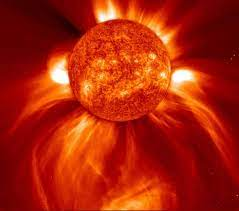
\includegraphics[width=0.5\textwidth]{Plasma.jpg}
\caption{\label{fig:Plasma } Plasma is the main constituent of Stars}
\end{figure}

\subsection{History, Discovery and its Source}
\begin{wrapfigure}{l}{0.35\textwidth}
    \centering
    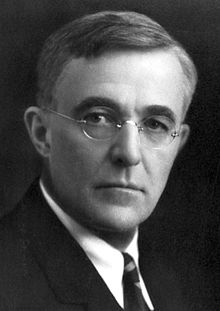
\includegraphics[width=0.2\textwidth]{Langmuir.jpg}
    \caption{\label{fig:Langmuir} Irving Langmuir} 
\end{wrapfigure}

The discovery of plasma as a distinct state of matter is attributed to the work of Irving Langmuir, an American chemist and physicist. In the early 20th century, Langmuir was studying the properties of gases at low pressures and discovered that by applying an electric current to a gas, he could create a new state of matter that was distinct from solids, liquids, and gases. This state was characterized by the presence of charged particles, such as ions and electrons, and was given the name "plasma" by Langmuir, who was inspired by the resemblance of the glowing gas to blood plasma.

\subsection{Properties}
\large
Plasma state is a highly dynamic system that can exhibit unique properties, such as the ability to conduct electricity, emit light, and generate magnetic fields.
\subsection{Types of Plasma}
 \begin{figure}[h]
\centering
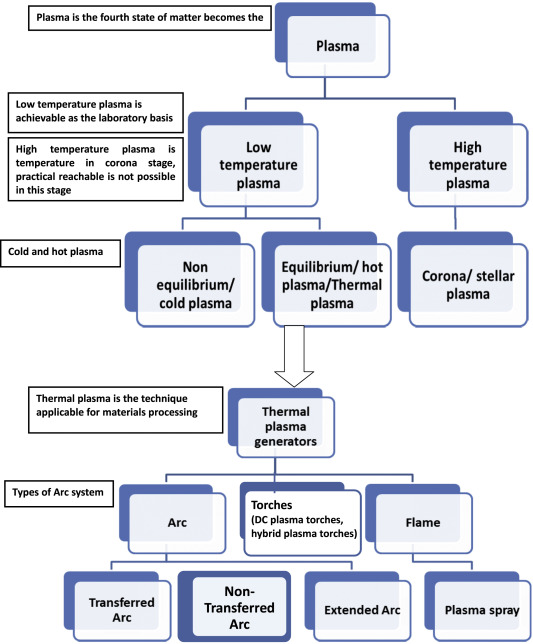
\includegraphics[width=0.5\textwidth]{Plasma Table.jpg}
\caption{\label{fig:Plasma Table } Classification of Plasma}
\end{figure}
Plasma can be classified into two main types based on the thermal conditions of the plasma with the surrounding environment: equilibrium and non-equilibrium plasma.
Understanding the differences between equilibrium and non-equilibrium plasma is important for designing and optimizing plasma-based technologies.

\subsubsection{Equilibrium Plasma}
Equilibrium plasma refers to a state where the plasma is in thermal equilibrium with its surroundings. This means that the temperature of the plasma is uniform and the same as the temperature of the surrounding gas or material. In equilibrium plasma, the number of charged particles, such as electrons and ions, is balanced, and there is no net charge in the plasma.
\subsubsection{Non- Equilibrium Plasma}

Non-equilibrium plasma, on the other hand, refers to a state where the plasma is not in thermal equilibrium with its surroundings. This means that the temperature of the plasma is not uniform and can be much hotter or colder than the surrounding gas or material. Non-equilibrium plasma is characterized by the presence of energetic electrons and ions, which can have a significant impact on the behavior of the plasma. Non-equilibrium plasma can be created by various methods, such as applying an electric field or using high-energy radiation.
\cite{10}
Non-equilibrium plasma has many unique properties that make it useful for a wide range of applications, such as in plasma cutting and welding, surface treatment, and plasma-based medicine. 


\section{Microwave Induced Plasma in Grapes}

This phenomenon occurs when a pair of grape hemispheres are exposed to intense microwave radiation, causing them to spark and ignite a plasma which is a low-temperature ionized gas that emits a variety of colorful and intriguing light spectra. 

\subsection{History}
\large
This experiment was published online in 1994 by 
\textbf{Patrick Michaud}

\subsection{\Large Physics Behind the Experiment}
\large
When the grape is placed in the microwave oven, the key thing is to observe how considerable the wavelengths are inside the grape.
The wavelength of the microwave inside the microwave oven is \textbf{12 cm}, whereas it is approximately \textbf{1.2 cm} inside the grape. Therefore, it can be observed that the wavelength of the microwave is \textbf{10 times} lesser in the grape compared to its wavelength in the air.
When we place the grape in the microwave oven and pass the microwave through it, the waves get trapped inside the grape. This is because the grape has a huge size and high refractive index.


\subsubsection{\large A Flaw in Previous Theories}
Until now, a general explanation was that the skin acted as a short dipole antenna and that the conducting ion-rich skin “bridge" played an important role. But till the recent past, there was not a correct explanation known until a recently published paper.\cite{3}

\subsubsection{\Large Total Internal Reflection}

\begin{wrapfigure}{l}{0.3\textwidth}
    
    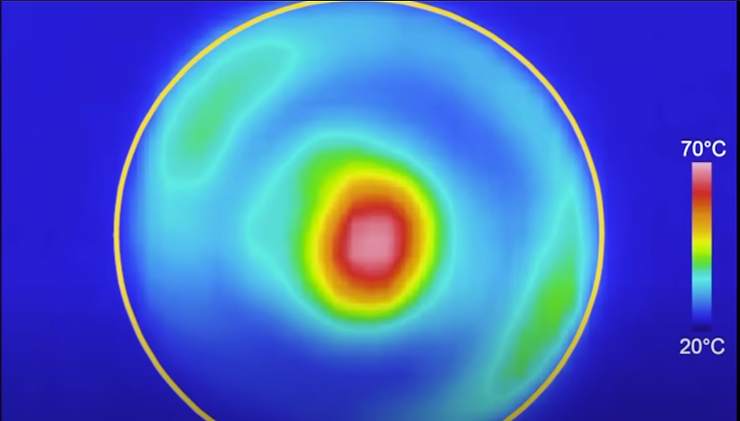
\includegraphics[width=0.25\textwidth]{Image-3.png}
   
\end{wrapfigure}
\Large
When we place the grape in the microwave oven and pass the microwave through it, the waves get trapped inside the grape. This is because the grape has a huge size and high refractive index.
And it starts bouncing inside. The microwave, unable to escape through the walls of the grape, starts to oscillate inside the grape and generate the maximum electromagnetic field at its center.
We expect the grape to heat from the outside, but in reality, it heats from the inside, as we can see in the figure.
\subsubsection{\Large Intersection of Two Grapes}

\begin{wrapfigure}{l}{0.3\textwidth}
    
    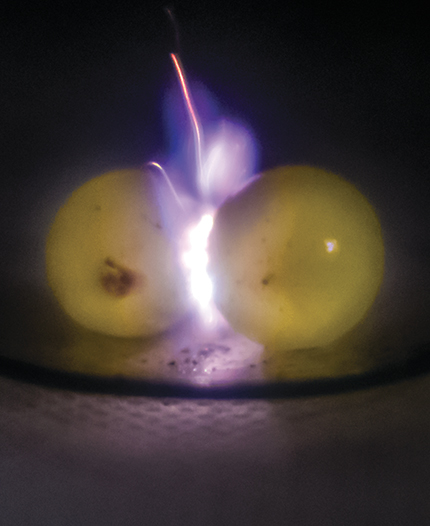
\includegraphics[width=0.2\textwidth]{m_96_1_f1.jpg}
   
\end{wrapfigure}
\Large

When we intersect the grapes and pass the microwave through it, the strongest oscillating electromagnetic field forms at the intersection point of the grapes.
We can catch sight of sparks at the intersection point of the grapes, i.e. the area with the strongest electromagnetic field. This is because the strong electric field ionizes the air, thus creating sparks. These sparks lead to the formation of plasma. The ions which are generated get more energy from the microwaves.






\subsection{\Large Experiment}

Science is all about \textbf{How and WHY}. And so experiments play an important role in Science learning.
Ordinary grapes, when properly prepared and microwaved, spark impressively in an extremely entertaining manner. So, let's try it. See, it’s not a very tough thing but yes, you need to be careful enough to prevent yourself from any harm.

\subsubsection{\Large Aim and Target}
\begin{itemize}
\item Using \textbf{cheap, readily-available equipment}, creating a spectacular light show in the kitchen
\item Promote \textbf{Interest, Love, and Excitement for Science} among budding and prospective School Students
\end{itemize}
\subsubsection{\Large Materials Required}
\begin{itemize}
\large
    \item A pack of Green Grapes. We may also use Hydrogel Water Beads to get the same results.
    \item Microwave Oven
    \item Plates that can withstand Microwave vibrations and won't crack
    \item Knife- For slicing the Grapes
    \item Camera or Mobile Phone to record the sparklings.
    
    
\end{itemize}

\subsubsection{\Large Procedure}
\large
\begin{itemize}
    \item Slice the grape such that the thin isthmus is still holding the two halves together.
    \begin{figure}[h]
        \centering
        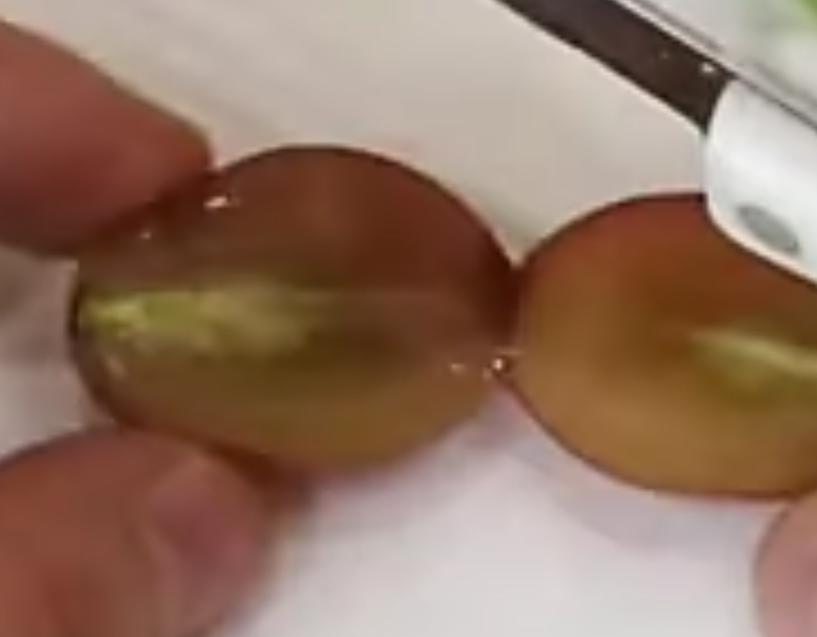
\includegraphics[width=0.3\textwidth]{Slicing the grapes with isthmus between.jpg}
        \caption{Slicing the grapes leaving an isthmus}
       
    \end{figure}
    \item Next, place them sliced side up.
    \begin{figure}[h]
\centering
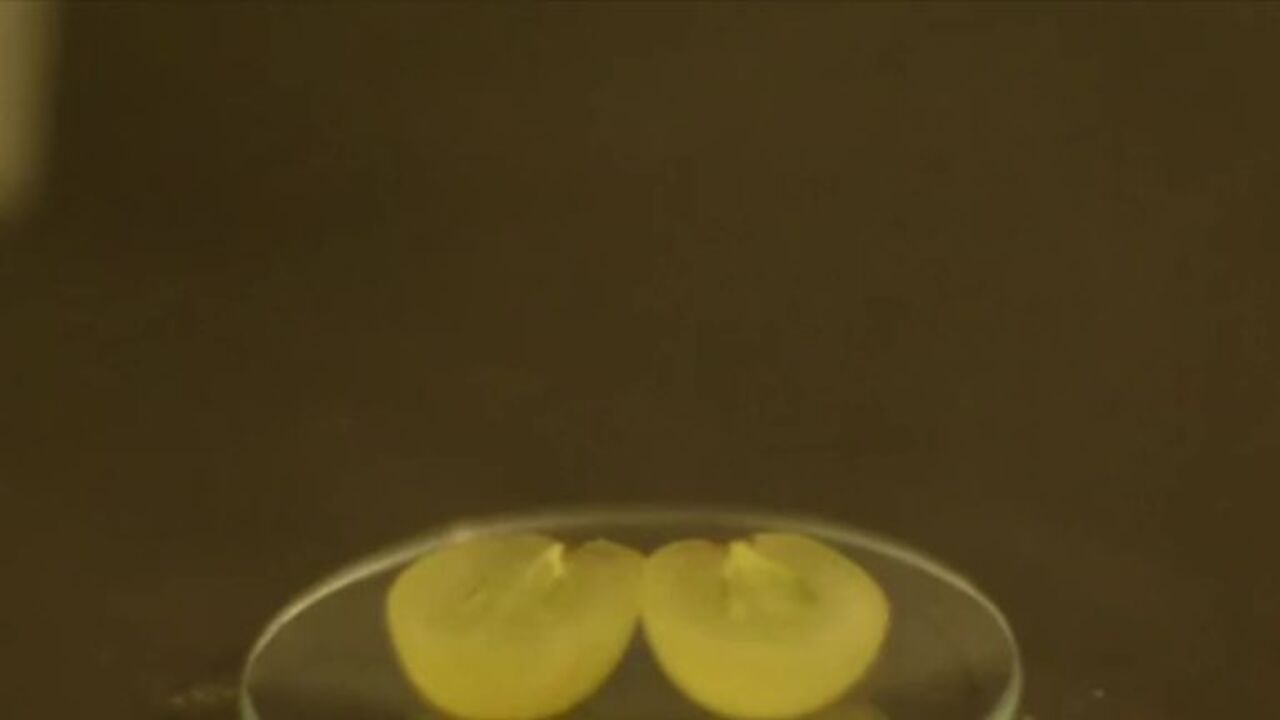
\includegraphics[width=0.5\textwidth]{sliced side up.jpg}
\caption{\label{fig:Grapes Sliced } Grapes Sliced side up}
\end{figure}

    \item  \large Place the plate with the prepared grapes into the center of the microwave oven and shut the door carefully. The microwave is set to cook at full power for 35-40 seconds.
    
    \item \large The sparks will start approximately 5 seconds after the microwave is started.
    \item \large Approximately 2-3 seconds after that, the force of the sparks separated the grape halves (the isthmus burns out) by approximately 1-1.5 cm, ending the effects. At this point, stop the microwave to prevent further damage.
    
    \begin{figure}
        \centering
        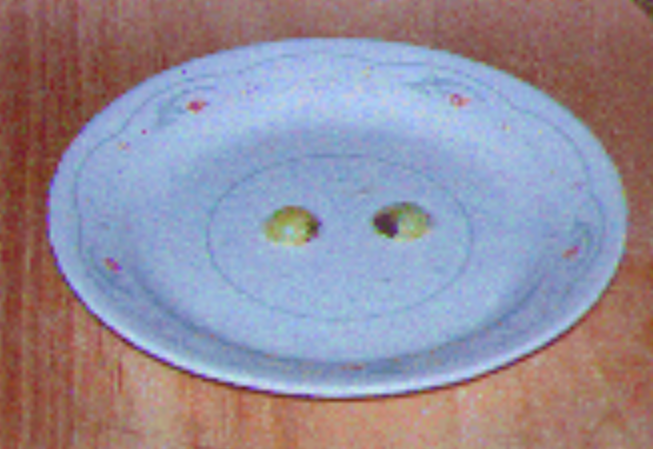
\includegraphics[width=0.3\textwidth]{After Sparkling.png}
        \caption{Slicing the grapes leaving an isthmus}
        \end{figure}
   
\end{itemize}

\subsubsection{\Large Results}
\large
We will see flares and sparks associated with the grapes as an effect of microwaves.

 \begin{figure}[h]
        \centering
        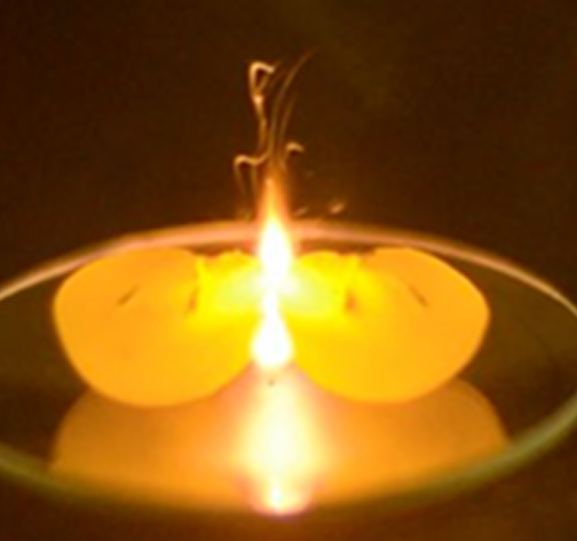
\includegraphics[width=0.5\textwidth ]{Grape-1.png}
        \caption{\label{fig:Sparkling Effects} Sparkling Flares in Grapes}
    \end{figure}



\subsection{Cases, Related Observations and Reasons }

We will extend our exploration a little further. Under the experiment section, we cut the grapes in slices such that we have a thin isthmus left. 
But here under this section, we'll not slice the grapes and instead will use two grapes, keep them in touch to see the effects.

\begin{figure}[h]
        \centering
        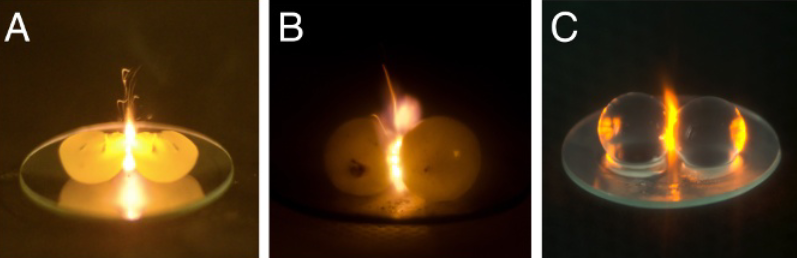
\includegraphics[width=0.6\textwidth]{Screenshot (504).png}
       \caption{ (A) Plasma between grape hemispheres bound with a skin bridge in the traditional arrangement. (B) Whole grapes, weakly bound by their weight in a watch glass, also form plasma.(C) Skinless hydrogel beads are $ > $  \SI{99}{\percent} and also form plasma after a brief immersion in \ce{NaCl} solution
       \cite{3} }
       
    \end{figure}
    In practice, as long as the grapes—or any other similarly sized pair of ion-rich aqueous spheres—are in contact, cutting is unnecessary. \cite{3} \textbf{Isolated spheres never spark}. Traditional explanations for the plasma formation almost invariably invoke a mechanism, such as surface plasmon* resonances, that relies on high surface conductivity, but new research is exploring bulk optical mechanisms such as \textbf{Mie resonances}. At 2.45 GHz, the typical frequency of consumer microwave ovens, water has a refractive index above 8 and relatively small absorption. That makes each grape, with a diameter of about 1.5 cm, the right size, composition, and shape for resonant scattering and produces a concentrated electric field at their point of contact.


\begin{figure}
        \centering
        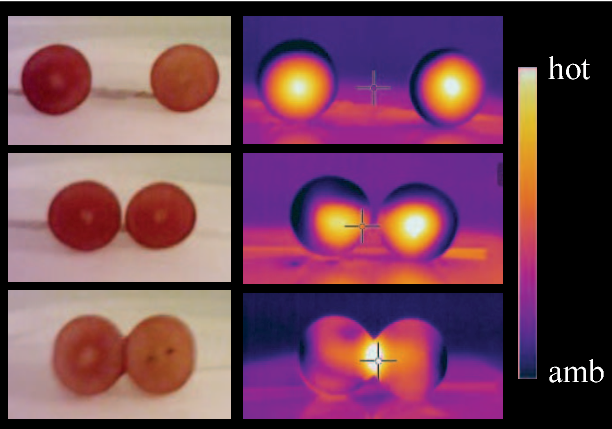
\includegraphics[width=0.5\textwidth]{1-Figure2-1.png}
       
    \end{figure}
    

\subsection{\Large Applications}
\begin{figure}[h]
        \centering
        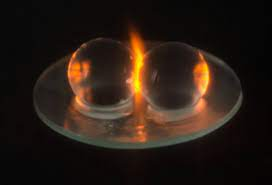
\includegraphics[width=0.5\textwidth ]{download (4).jpg}
     \label{fig:download (4)}
    \end{figure}
\large
\textbf{Microwave-induced Plasma} is a fascinating phenomenon and has attracted significant attention in the scientific community in recent years. 
Grape plasma has a lot of potential applications in fields such as agriculture, the food processing Industry, renewable energy, and Soft Robotics making it an exciting and intriguing area of researches 

\subsubsection{\Large Agriculture}

\large A study by \textbf{Michael, Babushok, and C. E. Dykstra} investigates the potential use of microwave-induced plasma in grape clusters for agricultural applications, such as plant disease control \cite{GDS}, \cite{PGTD} and pesticide residue removal. 
This technology is more environmentally friendly and energy-efficient than traditional chemical treatments, which can have negative impacts on the environment and human health. Moreover, it has the potential to improve crop yield and quality \cite{MIP}, reduce post-harvest losses, and increase food safety. 
Studies have demonstrated the effectiveness of using microwave-induced plasma in grape clusters for fruit surface sterilization\cite{SSGB}, and plant growth enhancement. Further research is required to optimize the technology for more practical applications in the agricultural industry.

\subsubsection{\Large Carbon Dioxide Methanation}
Carbon dioxide methanation process involves the reaction of carbon dioxide \ce{CO2} and hydrogen \ce{H2} to produce methane \ce{CH4}, which is a valuable fuel that can be used in various applications. The usual catalytic methanation process is energy-intensive and requires high temperatures and pressures. As an alternative approach, we can use \textbf{Microwave-induced grape plasma} for carbon dioxide methanation and is more energy-efficient and environmentally friendly. 
The use of microwave-induced grape plasma for carbon dioxide methanation has several advantages over traditional catalytic methanation. 
\begin{itemize}
    \item \normalsize The plasma process operates at lower temperatures and pressures, which reduces the energy requirements and the production of greenhouse gases
    \item \normalsize The plasma process can produce methane \ce{CH4} while traditional catalytic methanation can produce byproducts such as carbon monoxide \ce{CO} and water \ce{H20} .
    \item \normalsize The plasma process can operate at a smaller scale, which makes it suitable for distributed and decentralized applications
\end{itemize}

A study showed that microwave-induced grape plasma can effectively convert \ce{CO2} and \ce{H2} into \ce{CH4} at temperatures as low as \textbf {100°C} and pressures as low as \textbf {1 atm}.\cite{7}


\subsubsection{\Large Soft Robotics}
\large
When grapes are irradiated in a microwave oven, an intense electromagnetic hotspot forms at their point of contact, igniting flames and sparks, our Plasma. So, according to the research by \textbf{Hamza K. Khattak, R. Waitukaitis, Aaron D. Slepkov},\cite{4} we see that this irradiation can result in the injection of mechanical energy. By examining this, through high-speed imaging, we find that they repeatedly bounce off of each other while irradiated. We can see and confirm this statement from the YouTube videos. (An Extensive List is provided under the \textbf{References} Section)


\begin{figure}[h]
        \centering
        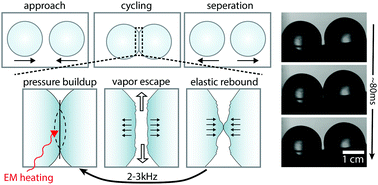
\includegraphics[width=0.5\textwidth ]{Image-4.png}
        \caption{\cite{4}}
        
     \label{fig:}
    \end{figure}

It was determined that an average of 1 $\mu J $ of mechanical energy is injected into the pair during each collision. Also, a high-pitched audio signal is found to accompany each collision. We show that both the audio signal and the energy injection arise via an interplay between vaporization and elastic deformations in the region of contact, the so-called ‘\textbf {elastic Liedenfrost effect}".
So, \textbf {Elastic Liendefrost} refers to the phenomenon of droplets bouncing on a surface due to the formation of an air cushion beneath them.
So, It has applications in the field of \textbf{Soft Robotics}.
\begin{figure}[h]
        \centering
        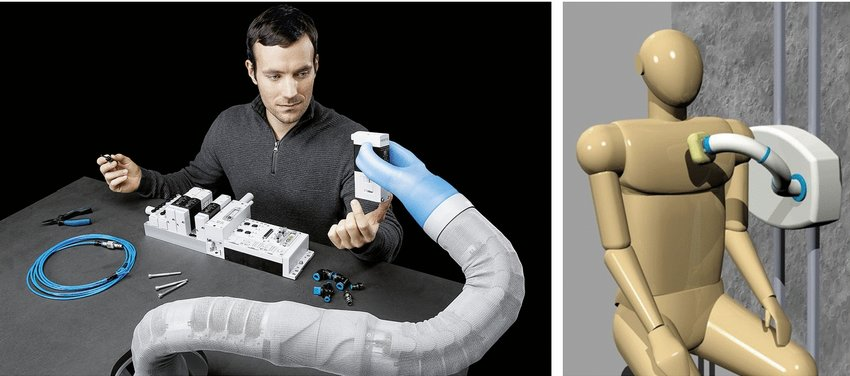
\includegraphics[width=0.5\textwidth ]{Soft Robots.png}
        \caption{\label{fig: Soft Robots}
        \footnotesize Examples of soft robots based on tentacle designs developed for scenarios that involve close interaction with humans: the Festo BionicSoftArm cobot (left) and the I-SUPPORT system for assisted bathing (right).\cite{2}}
    \end{figure}

\subsubsection{\large Potential Applications}
Some of the special characteristics of \textbf{Microwave-Induced Plasma in Grapes} have the potential to be a versatile and efficient tool for various applications in the fields of
\begin{itemize}
    
   
    \item \textbf{ Bio-medicine}
    \item \textbf{ Tip-enhanced near-field microscopy}
    \item \textbf{ Lithographic Techniques}
    \item \textbf{ Fabrication of Semiconductor Microchips}
    \item \textbf{ Omnidirectional Antenna Design}
    \item \textbf{ Food sterilization}:  {Plasma can be used to sterilize food and reduce the risk of contamination by pathogens such as bacteria and viruses. Microwave-induced grape plasma effectively reduces the levels of microorganisms making it a potential alternative to traditional sterilization methods such as heat treatment.}
    \item \textbf{{Material processing}}: {Microwave-induced grape plasma has been shown to enhance the adhesion of coatings on metals  and improve the surface roughness of polymers.}
    
    

\end{itemize}




\subsection{Bibliography and References}

Here, you will get an extensive list of resources and references I've used and read while making this Document.

\bibliographystyle{alpha}
\bibliography{sample}




\end{document}
